\documentclass[9pt]{beamer}

\beamertemplatenavigationsymbolsempty
\renewcommand\mathfamilydefault{cmr}

\usepackage{xcolor}
\usepackage{pajmath}
\usepackage{booktabs}
\usepackage{colortbl}
\usepackage{tikz}
\usetikzlibrary{calc}
\usetikzlibrary{intersections}
\usetikzlibrary{datavisualization}
\usetikzlibrary{datavisualization.formats.functions}
\usepackage{pgfplots}

\newcommand\VW{\V{W}}
\newcommand\bsigma{\boldsymbol{\sigma}}

\title{Neural Networks: Multi-layer Perceptrons}
\date{Spring 2021}

\begin{document}

\maketitle

\begin{frame}{Review}

\begin{itemize}
	\item A perceptron is a simplistic model of a single neuron.
	\item A perceptron can learn to perform simple classification tasks using an update rule.
	\item \textbf{Today:} Imagine what a network of millions of perceptrons can learn!
\end{itemize}
	
\end{frame}

\begin{frame}{A new activation function}

Our simple perceptron computes an intermediate value $z$ using a weighted sum of the inputs
\[ z = \V{w}\cdot\Vx \]
To simulate firing, we used the \emph{sign function} for activation:
\[ 
	y = \mathrm{sgn}(z) = \begin{cases} +1, & z > 0 \\ -1, & z < 0 \end{cases} \quad
	\raisebox{-0.45in}{
		\begin{tikzpicture}
			\draw [help lines,->] (-1,0) -- (1,0) node [below] {$z$};
			\draw [help lines,->] (0,-1) -- (0,1) node [left] {$y$};
			\draw [thick,blue] (-1,-1) node [left] {$-1$} -- (0,-1) (0,1) -- (1,1) node [right] {$+1$};
		\end{tikzpicture}
	}
\]
To avoid the discontinuity at zero, let's switch to the \emph{sigmoid function}:
\[ 
	y = \sigma(z) = \frac{1}{1 + e^{-z}} \quad
	\raisebox{-0.3in}{
		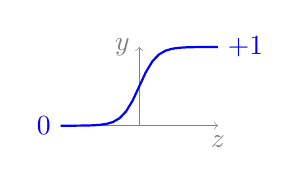
\begin{tikzpicture}
			\draw [help lines,->] (-1,0) -- (1,0) node [below] {$z$};
			\draw [help lines,->] (0,0) -- (0,1) node [left] {$y$};
			\draw [thick,blue, xscale=0.111, domain=-9:9] plot (\x, {1/(1+exp(-\x)});
			\node [blue,left] at (-1,0) {$0$};
			\node [blue,right] at (1,1) {$+1$};
		\end{tikzpicture}
	}
\]

\end{frame}

\begin{frame}{Back to logistic regression?}

A perceptron with a sigmoid activation function
\[ y = \sigma(\V{w}\cdot\Vx) \]
is equivalent to a logistic regression model.

\pause
\bigskip
Adding the sigmoid function prevents us from using the Perceptron Update Algorithm. We must use a gradient descent-type method instead (just as we did for logistic regression).

\bigskip
Fortunately, the sigmoid function has a convenient derivative:
\[ \frac{d}{dz}\sigma(z) = \sigma(z)[1 - \sigma(z)]. \]
	
\end{frame}

\begin{frame}{Multi-neuron (wide) perceptrons}

Neural networks use multiple neurons to learn different features from the \textbf{same inputs}.

\begin{center}
	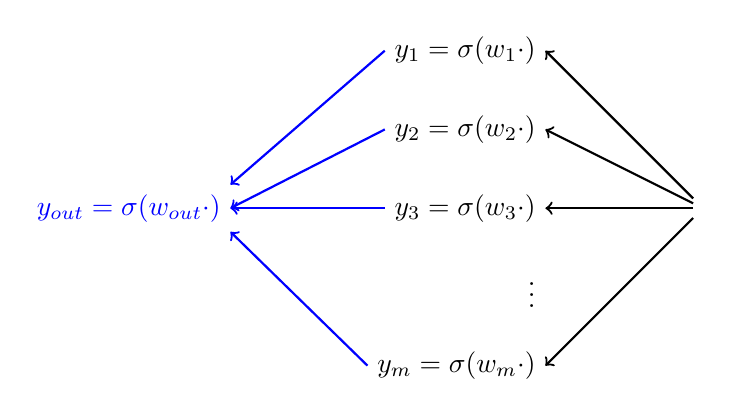
\begin{tikzpicture}
		\node [left] (a) at (0,3) {$y_1 = \sigma(\V{w}_1\cdot\Vx)$};
		\node [left] (b) at (0,2) {$y_2 = \sigma(\V{w}_2\cdot\Vx)$};
		\node [left] (c) at (0,1) {$y_3 = \sigma(\V{w}_3\cdot\Vx)$};
		\node [left] (d) at (0,0) {$\vdots$};
		\node [left] (e) at (0,-1) {$y_m = \sigma(\V{w}_m\cdot\Vx)$};
		\node (s) at (2,1) {$\Vx$};
		\draw [->,thick] (s) -- (a.east);
		\draw [->,thick] (s) -- (b.east);
		\draw [->,thick] (s) -- (c.east);
		\draw [->,thick] (s) -- (e.east);
		\onslide<2->{
			\node [blue,left] (o) at (-4,1) {$y_\text{out} = \sigma(\V{w}_\text{out}\cdot\Vy)$};
			\draw [->,blue,thick] (a.west) -- (o.north east);
			\draw [->,blue,thick] (b.west) -- (o.east);
			\draw [->,blue,thick] (c.west) -- (o.east);
			\draw [->,blue,thick] (e.west) -- (o.south east);
		};
	\end{tikzpicture}
\end{center}

\onslide<2->{
	The outputs of each neuron are collected into a single output neuron to predict the final class.
}

\end{frame}

\begin{frame}{A matrix formalism for perceptrons}

Consider a stack of $m$ neurons that are all connected to the same input~\Vx.
\begin{align*}
	z_1 &= \V{w}_1\cdot\Vx \\
	z_2 &= \V{w}_2\cdot\Vx \\
	 &\vdots \\
	z_m &= \V{w}_m\cdot\Vx \\
\end{align*}

\pause
The stack can be written as the product of the input~\Vx\ and a weight matrix
\[ \Vz = \V{W}\Vx \]
where each row in $\V{W}$ contins the weights for a single neuron
\[ \V{W} = \begin{pmatrix} \leftarrow \V{w}_1 \rightarrow \\
 						   \leftarrow \V{w}_2 \rightarrow \\
 						    \vdots \\
 						   \leftarrow \V{w}_m \rightarrow \\	
 \end{pmatrix}. \]
	
\end{frame}

\begin{frame}{Three looks at linear systems}

We've studied three classes of linear systems, differing only by what is \textbf{known} and {\color{red}\textbf{unknown}}.

\bigskip
\large
\begin{align*}
	{\color{red}\Vy} &= \VA\Vx && \text{matrix multiplication} \\
	\Vy &= \VX{\color{red}\Vbeta} && \text{linear models} \\
	\Vz &= {\color{red}\V{W}}\Vx && \text{neural networks}
\end{align*}

\pause
\bigskip
\normalsize
Of these problems, neural networks are the most difficult to solve since $\V{W}$ is a \emph{matrix} of unknowns, not a \emph{vector} like \Vy\ and $\Vbeta$.
	
\end{frame}

\begin{frame}{Elementwise activation functions}

Let's define an \emph{elementwise} sigmoid activation function
\[ \bsigma(\Vz) = \begin{pmatrix} \sigma(z_1) \\ \sigma(z_2) \\ \vdots \\\sigma(z_n) \end{pmatrix}. \]
	
\pause
A stack of $m$ neurons can be written as
\begin{align*}
	\Vz &= \V{W}\Vx \\
	\Vy &= \bsigma(\Vz)	
\end{align*}
\pause
or, more succinctly as
\[ \Vy = \bsigma(\V{W}\Vx) \]
\pause
where
\[ \dim(\Vy)=m\times 1,\quad \dim(\Vz)=m\times 1 \]
\[ \dim(\V{W})=m\times n,\quad \dim(\Vx)=n\times 1 \]
\end{frame}

\begin{frame}{Completing our matrix formalism}
\begin{center}
	\small
	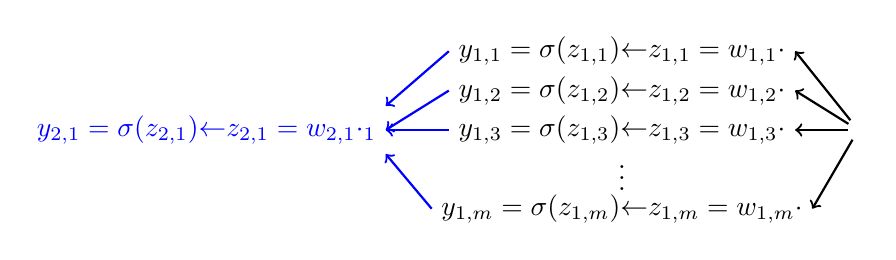
\begin{tikzpicture}
		\node (a) at (0,1.5) {$y_{1,1} =\sigma(z_{1,1}) \boldsymbol{\leftarrow} z_{1,1} = \V{w}_{1,1}\cdot\Vx$};
		\node (b) at (0,1) {$y_{1,2} =\sigma(z_{1,2}) \boldsymbol{\leftarrow} z_{1,2} = \V{w}_{1,2}\cdot\Vx$};
		\node (c) at (0,0.5) {$y_{1,3} =\sigma(z_{1,3}) \boldsymbol{\leftarrow} z_{1,3} = \V{w}_{1,3}\cdot\Vx$};
		\node (d) at (0,0) {$\vdots$};
		\node (e) at (0,-0.5) {$y_{1,m} =\sigma(z_{1,m}) \boldsymbol{\leftarrow} z_{1,m} = \V{w}_{1,m}\cdot\Vx$};
		\node (s) at (3,0.5) {$\Vx$};
		\draw [->,thick] (s) -- (a.east);
		\draw [->,thick] (s) -- (b.east);
		\draw [->,thick] (s) -- (c.east);
		\draw [->,thick] (s) -- (e.east);
		\node [blue,left] (o) at (-3,0.5) {$y_{2,1} =\sigma(z_{2,1}) \boldsymbol{\leftarrow} z_{2,1} = \V{w}_{2,1}\cdot\Vy_1$};
		\draw [->,blue,thick] (a.west) -- (o.north east);
		\draw [->,blue,thick] (b.west) -- (o.east);
		\draw [->,blue,thick] (c.west) -- (o.east);
		\draw [->,blue,thick] (e.west) -- (o.south east);
	\end{tikzpicture}
\end{center}

\[  \Vy_2 = \bsigma(\Vz_2) \quad\leftarrow\quad
	\Vz_2 = \V{W}_2\Vy_1 \quad\leftarrow\quad
	\Vy_1 = \bsigma(\Vz_1) \quad\leftarrow\quad
	\Vz_1 = \V{W}_1\Vx	 \]

\[ \Vy_2 = \bsigma(\V{W}_2(\bsigma(\V{W}_1\Vx))) \]

\[ \Vy_d = \bsigma(\V{W}_d(\bsigma(\V{W}_{d-1}(\cdots\bsigma(\V{W}_2(\bsigma(\V{W}_1\Vx))))))) \]

\end{frame}

\begin{frame}{Deep learning with neural networks}

\[ \Vy_d = \bsigma(\V{W}_d(\bsigma(\V{W}_{d-1}(\cdots\bsigma(\V{W}_2(\bsigma(\V{W}_1\Vx))))))) \]

\bigskip
\begin{itemize}
	\item The number of neurons in each layer $i$ is the \emph{width} of the layer.
	\begin{itemize}
		\item If the ($i-1$)th layer has $n$ outputs and the $i$th layer has $m$ outputs, the weight matrix $\V{W}_i$ has dimensions $m\times n$.
		\item The dimensions of the inputs \Vx\ and outputs $\Vy_d$ are fixed by the problem.
		\item Layer $1$ is called the \emph{input layer}, and layer $d$ is the \emph{output layer}.
		\item We can use as many nodes as we want in the \emph{hidden} layers.
	\end{itemize}
	\item<2-> The number of layers $d$ in the \emph{depth} of the neural network.
	\item<3-> \emph{Deep learning} means $d>2$.
\end{itemize}
	
\end{frame}

\begin{frame}{The importance of nonlinearity}

The nonlinear functions (like $\bsigma$) sandwiched between the layers are critical to deep learning.

\bigskip
Let's imagine what would happen if we removed them:
\begin{align*}
	\Vy_d &= \bsigma(\V{W}_d(\bsigma(\V{W}_{d-1}(\cdots\bsigma(\V{W}_2(\bsigma(\V{W}_1\Vx))))))) \\
		 &= \V{W}_d(\V{W}_{d-1}(\cdots\V{W}_2(\V{W}_1\Vx))) \\
		 &= \V{W}_d \V{W}_{d-1} \cdots \V{W}_2 \V{W}_1 \Vx \\
		 &= \widetilde{\V{W}}\Vx
\end{align*}

\pause
\bigskip
Without the activation functions, the entire neural network reduces to a single linear system!
	
\end{frame}

\begin{frame}{Any nonlinearity will do}

Any nonlinear function can be an activation function.

\begin{columns}[T]
\begin{column}{0.3\textwidth}
	\begin{center}
		\textbf{Sign/step activation}
	\end{center}
\end{column}	
\begin{column}{0.3\textwidth}<2->
	\begin{center}
		\textbf{Sigmoid activation}
	\end{center}
\end{column}	
\begin{column}{0.3\textwidth}<3->
	\begin{center}
		\textbf{Rectified linear unit activation}
	\end{center}
\end{column}	
\end{columns}

\begin{columns}[T]
\begin{column}{0.3\textwidth}
	\begin{center}
		\[ \mathrm{sgn}(z) = \begin{cases} +1, & z > 0 \\ -1, & z < 0 \end{cases} \]
	\end{center}
\end{column}	
\begin{column}{0.3\textwidth}<2->
	\begin{center}
		\[ \sigma(z) = \frac{1}{1 + e^{-z}} \]
	\end{center}
\end{column}	
\begin{column}{0.3\textwidth}<3->
	\begin{center}
		\[ \mathrm{ReLU}(z) = \begin{cases} z, & z \ge 0 \\ 0, & z < 0 \end{cases} \]
	\end{center}
\end{column}	
\end{columns}


\begin{columns}[T]
\begin{column}{0.3\textwidth}
	\begin{center}
		\begin{tikzpicture}
			\draw [help lines,->] (-1,0) -- (1,0) node [below] {$z$};
			\draw [help lines,->] (0,-1) -- (0,1) node [left] {$y$};
			\draw [thick,blue] (-1,-1) node [left] {$-1$} -- (0,-1) (0,1) -- (1,1) node [right] {$+1$};
		\end{tikzpicture}
	\end{center}
\end{column}

\pause
\begin{column}{0.3\textwidth}<2->
	\begin{center}
		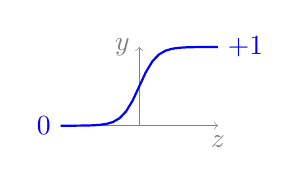
\begin{tikzpicture}
			\draw [help lines,->] (-1,0) -- (1,0) node [below] {$z$};
			\draw [help lines,->] (0,0) -- (0,1) node [left] {$y$};
			\draw [thick,blue, xscale=0.111, domain=-9:9] plot (\x, {1/(1+exp(-\x)});
			\node [blue,left] at (-1,0) {$0$};
			\node [blue,right] at (1,1) {$+1$};
		\end{tikzpicture}
	\end{center}
\end{column}

\pause
\begin{column}{0.3\textwidth}<3->
	\begin{center}
		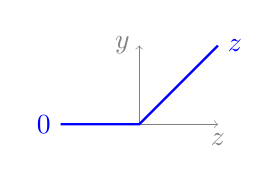
\begin{tikzpicture}
			\draw [help lines,->] (-1,0) -- (1,0) node [below] {$z$};
			\draw [help lines,->] (0,0) -- (0,1) node [left] {$y$};
			\draw [thick,blue] (-1,0) -- (0,0) -- (1,1);
			\node [blue,left] at (-1,0) {$0$};
			\node [blue,right] at (1,1) {$z$};
		\end{tikzpicture}
	\end{center}
\end{column}

\end{columns}	
\end{frame}

\begin{frame}{Preparing for gradient descent}

Neural networks are trained with a variation of gradient descent. Before calculating the gradients, we need to review the chain rule from calculus.

\bigskip
\pause
For any differentiable functions $f$ and $h$,
\[ \frac{d}{dx}h(f(x)) = \frac{dh}{df}\frac{df}{dx} \]

\pause
Similarly, for the $k$ functions $f_1$, $f_2$, $\ldots$, $f_k$,
\[ \frac{d}{dx}f_k(f_{k-1}(\cdots f_2(f_1(x)))) = \frac{df_k}{df_{k-1}} \frac{df_{k-1}}{df_{k-2}}\cdots \frac{df_i}{df_{i-1}}\cdots \frac{df_2}{df_1}\frac{df_1}{dx} \]

\pause
For example, let $f(x) = (2x-3)^3$. Let $f_1(x) = 2x-3$ and $f_2(z) = z^3$. Then $f(x) = f_2(f_1(x))$ and
\begin{align*}
	\frac{df}{dx} &= \frac{df_2}{df_1}\frac{df_1}{dx} \\
		&= 3(2x-3)^2(2)
\end{align*}
\end{frame}

\begin{frame}{Backpropagation through neural networks}

Let's assume we have some loss function $L$ that measures how well the output of the final layer ($y_d$) compared with known training data.

\bigskip
\pause
The loss function depends on all the weights in the network, i.e.\ $L(\V{W}_d,\V{W}_{d-1},\ldots,\V{W}_2,\V{W}_1)$.

\bigskip
\pause
To update the weights, we need to calculate the partial derivatives
\[ \dd{L}{\V{W}_i},\quad i=1\ldots d \]
	
\end{frame}

\begin{frame}{Backpropagation through neural networks: The chain rule}

Let's use a 2-layer network $d=2$:
\[ \Vy_2 = \bsigma(\VW_2(\bsigma(\VW_1\Vx))) \]
which we can expand to
\begin{align*}
	 \Vy_2 &= \bsigma(\Vz_2) \\
	 \Vz_2 &= \VW_2\Vy_1 \\
	 \Vy_1 &= \bsigma(\Vz_1) \\
	 \Vz_1 &= \VW_1\Vx
\end{align*}

\begin{align*}
	\dd{\Vy_2}{\VW_2} &= \dd{Vy_2}{\Vz_2} \dd{\Vz_2}{\VW_2} \\
					  &= \bsigma' \Vy_1
\end{align*}

\begin{align*}
	\dd{\Vy_2}{\VW_1} &= \dd{\Vy_2}{\Vz_2} \dd{\Vz_2}{\Vy_1} \dd{\Vy_1}{\Vz_1} \dd{\Vz_1}{\Vx} \\
					  &= \bsigma' \VW_2 \bsigma' \Vx
\end{align*}

	
\end{frame}



\end{document}
